\documentclass[preview]{standalone}

\usepackage{amsmath}
\usepackage{amssymb}
\usepackage{stellar}
\usepackage{definitions}
\usepackage{bettelini}

\begin{document}

\id{matematica-dimostrazioni}
\genpage

\section{Teorema di Pitagora}

\begin{snippettheorem}{teorema-di-pitagora}{Teorema di Pitagora}
  Il teorema di Pitagora afferma che la somma del quadrato dei cateti di un triangolo rettangolo
  equivale al quadrato dell'ipotenusa
  \[
    a^2 + b^2 = c^2
  \]
\end{snippettheorem}

\begin{snippetproof}{teorema-di-pitagora-dimostrazione}{teorema-di-pitagora}{Teorema di Pitagora}
    Costruendo un quadrato utilizzando un triangolo rettangolo qualsiasi ripetuto quattro volte,
    si può ottenere la seguente rappresentazione

    \vspace{0.5cm}

    \begin{center}
        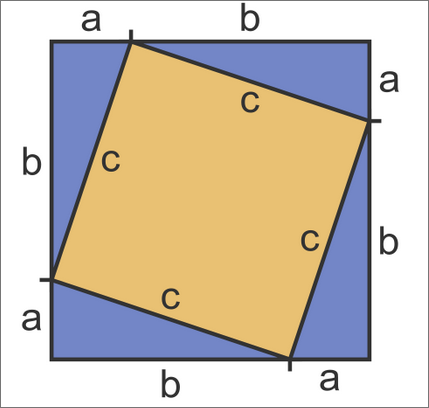
\includegraphics[width=0.2\textwidth]{resources/pythagorean-theorem-proof.png}
    \end{center}

    \vspace{0.5cm}

    L'area del quadrato esterno è data da \( (a + b)^2 \), ma anche da \( \frac{a \cdot b}{2} \cdot 4 + c^2\), da questo
    si può quindi stabilire la seguente uguaglianza:
    \[ 
       (a + b)^2 = \frac{a \cdot b}{2} \cdot 4 + c^2
    \]
    che si può semplificare
    \[ 
      a^2 + 2ab + b^2 = 2ab + c^2 
    \]
    \[ 
      a^2 + b^2 = c^2
    \]
\end{snippetproof}

\section{Somma degli angoli interni di un triangolo}

\section{Quadrato di numero dispari è dispari}

\end{document}
